\documentclass[12pt]{article}


\usepackage{hyperref}
\usepackage[width=6in,height=8in]{geometry}
\usepackage{guitardiagrams}
\usepackage{graphicx}
\usepackage{float}

\usepackage{amsthm}
\theoremstyle{definition}
\newtheorem{exercise}{Exercise}


\title{Left/Right Movable Scale Patterns}
\author{Addison Ballif}
\date{\today}

\begin{document}

\maketitle

In this document I describe a system for movable scale patterns on the guitar. Movable scale patterns are scale patterns that do not involve open strings. 
The advantage of using movable scale patterns is that they are not specific to a given key. 

The goal of this document is to teach you a system for playing scales that should open up the fretboard for you in melody playing and soloing. 
This system breaks all major scales into two types. We will call them the ``left'' type and the ``right'' type based on which side of the hand they start on. 
\begin{figure}[H]
\centering
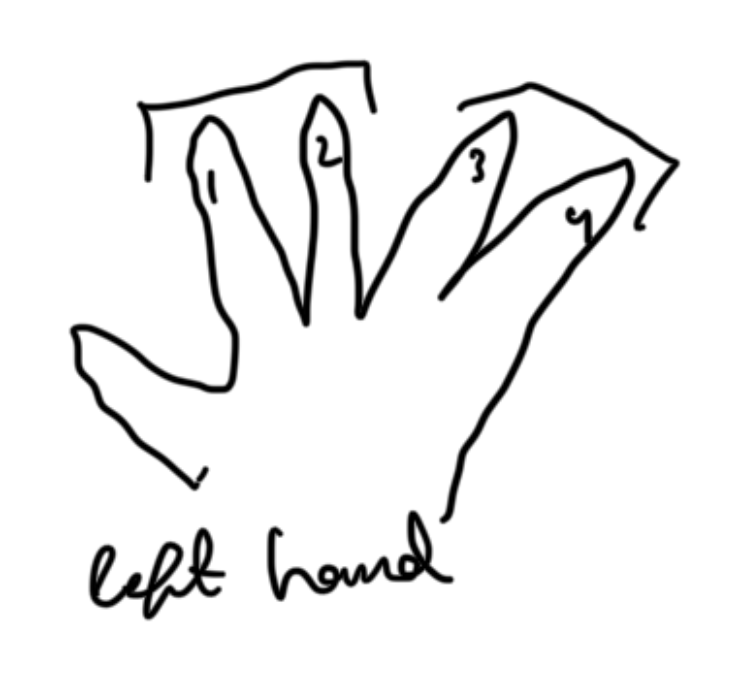
\includegraphics[width=0.3\linewidth]{hand_figure.png}
\caption{The left hand is split into two sides.}
\end{figure}
If a scale pattern starts with either of the first two fingers (1 or 2), then it will be called a ``left'' type scale, and if it starts on the right two fingers (3 or 4), it will be called a ``right'' type scale.

\section{Left Type Major Scales}
In this section I describe the left type major scale pattern. 
Scale patterns will look slightly different depending on what string they start on, but hopefully you can see that four left type major scales starting on each string are very similar to each other. This is why we describe them as being the same pattern. 

Starting on the low E string, the left type major scale is shown below. 

\fretboard[frets=4]{
    1/2/{R},
    1/4/{},
    2/1/{},
    2/2/{},
    2/4/{},
    3/1/{},
    3/3/{},
    3/4/{R}
}
The R represents the root of the major scale. 
To play this pattern, start with your middle finger (finger 2), and place your hand on the neck so that you have one finger per fret. 

We use this scale by starting R on the key of the scale we are trying to play. For example, if you want to play a G major scale, you would start this scale pattern with the bottom R on fret 3. 

\begin{exercise}
Play the following major scales starting on the E string in this order: A, C, G, B$\flat$, F$\sharp$. Start on the bottom note and play each note up to the top note. Then go back down. 
\end{exercise}

When playing this scale pattern on the A string it looks exactly the same. 

\fretboard[frets=4]{
    2/2/{R},
    2/4/{},
    3/1/{},
    3/2/{},
    3/4/{},
    4/1/{},
    4/3/{},
    4/4/{R}
}

Similar to the previous, we choose the key for the major scale by where we start. For example, if we wanted to play a D major scale, we would start on fret 5. 

\begin{exercise}
Play the following major scales starting on the A string in this order: E$\flat$, G, C, F.
\end{exercise}

When we move to the D string, the scale looks a little bit different. The top string of the pattern is shifted up. 

\fretboard[frets=5]{
    3/2/{R},
    3/4/{},
    4/1/{},
    4/2/{},
    4/4/{},
    5/2/{},
    5/4/{},
    5/5/{R}
}

To play this one, we shift our hand up a fret when we get to that top string. To check, the order of fingers used should be 2-4-1-2-4-1-3-4, the same as the previous two. The only thing that changes is that our hand shifts up when we get to the higher string. 

\begin{exercise}
Play the following major scales starting on the D string in this order: A, C, G, B$\flat$, F$\sharp$.
\end{exercise}

The previous three scale patterns have all started with the second finger. When we move the pattern up one more string, we will have to start on the first finger instead. However, the shape of the pattern is still very similar. 

\fretboard[frets=4]{
    4/1/{R},
    4/3/{},
    5/1/{},
    5/2/{},
    5/4/{},
    6/1/{},
    6/3/{},
    6/4/{R}
}

Start the scale with your index finger (finger 1). The order of fingers used should be 1-2-1-2-3-1-3-4. This is the same as the previous four patterns except for the first two notes. 

\begin{exercise}
Play the following major scales starting on the G string in this order: E$\flat$, G, C, F, B$\flat$.
\end{exercise}

Now you know all four of the left type major scales, you can start to play in different places over the fretboard and in any key! The following exercise gives a good way to practice these scale patterns. 

\begin{exercise} \label{ex:randomkey1}
Pick a random key. Then for each of the first four strings (E, A, D, G) play the major scale using the left type major scale pattern. Start on the bottom note and play to the top of the scale pattern. Then come back down. 
\end{exercise}

It is useful to do this exercise over a drone.\footnote{There is a page on my website that has drones in every key. It can be found \href{https://ahballif.github.io/AddisonGuitarResources/drones.html}{here.}}
This helps you internalize the sound of the scale as you practice. 
When playing over a drone, you may choose to ``noodle around'' the scale to experiment with what the different scale degrees sound like against the sound of a drone. 

It is also very useful to practice with a metronome.\footnote{The drone page on my website also has a metronome you can use. }
You might practice with 2 notes per click, or 4 notes per click. Being able to play with a metronome is a essential skill to learn. 

\section{Right Type Major Scales}
In this section I will teach you the other type of major scale patterns. These scales start on the right side of the hand. Similar to the previous section, these four scale patterns are nearly identical with slight modifications depending on which string you start on. They also can be placed anywhere on the neck to give the desired major scale. 

First we have the scale pattern starting on the low E string. This scale pattern starts with the pinkie finger (finger 4). 
Similar to previous, we will place one finger per fret. You will notice that on the last two notes, the hand needs to be shifted down a fret to play the note with the index finger (finger 1) and the middle finger (finger 2).

\fretboard[frets=5]{
    1/5/{R},
    2/2/{},
    2/4/{},
    2/5/{},
    3/2/{},
    3/4/{},
    4/1/{},
    4/2/{R}
}
The order of fingers used should be 4-1-3-4-1-3-1-2.

\begin{exercise}
Play the following major scales starting on the low E using the right type scale pattern in this order: C, A, E$\flat$, B$\flat$.
\end{exercise}

The scale pattern for the A string is mostly the same, except we no longer need to shift to reach the top two tones. 
\fretboard[frets=4]{
    2/4/{R},
    3/1/{},
    3/3/{},
    3/4/{},
    4/1/{},
    4/3/{},
    5/1/{},
    5/2/{R}
}

\begin{exercise}
Play the following major scales starting on the A string using the right type scale pattern in this order: D, G, E$\flat$, F$\sharp$.
\end{exercise}

The scale pattern for the D string is given below.
\fretboard[frets=4]{
    3/4/{R},
    4/1/{},
    4/3/{},
    4/4/{},
    5/2/{},
    5/4/{},
    6/1/{},
    6/2/{R}
}
Notice that this time the fingerings do change a little bit in order to keep one finger per fret. The order of fingers used should be 4-1-3-4-2-4-1-2. 

\begin{exercise}
Play the following major scales starting on the D string using the right type scale pattern in this order: B$\flat$, G, C, A$\flat$.
\end{exercise}

The last scale pattern (starting on the G string) only plays the first half of the major scale. We will see more how to play the rest with this pattern later. For now, just play to the top of the scale pattern and then go back down. 

The other difference with this scale pattern is that it starts on the ring finger (finger 3) instead of the pinkie finger. This preserves the one finger per fret spacing. 

\fretboard[frets=4]{
    4/3/{R},
    5/1/{},
    5/3/{},
    5/4/{},
    6/1/{},
    6/3/{}
}

The order of fingers used should be 3-1-3-4-1-3. 

\begin{exercise}
Play the following major scales (first 6 notes) starting on the G string using the right type scale pattern in this order: C, F, D.
\end{exercise}

We are now able to expand Exercise \ref{ex:randomkey1} to include both scale patterns. 

\begin{exercise} \label{ex:randomkey2}
Pick a random key. Then for each of the first four strings (E, A, D, G) play the major scale using the left type major scale pattern. Then do the same using the right type major scale pattern. 
\end{exercise}

\section{Combining Both Patterns}
By now you may have noticed that if a scale pattern starts on the left side of the hand, it will end on the right side of the hand, and vise-versa. This powerful pattern is what will allow us to play across the octave, meaning from one octave to the octave above. 

Consider the two octave major scale shown below. 

\fretboard[frets=4]{
    1/2/{R},
    1/4/{},
    2/1/{},
    2/2/{},
    2/4/{},
    3/1/{},
    3/3/{},
    3/4/{R},
    4/1/{},
    4/3/{},
    4/4/{},
    5/2/{},
    5/4/{},
    6/1/{},
    6/2/{R}
}

This scale pattern starts using the left type pattern on the low E string. When it gets to the octave it lands on figure 4, which sets it up to use the right type pattern. It then uses the right type pattern to go to the second octave. 

\begin{exercise}
Play the two octave major scale shown above in the following keys: G, C, B$\flat$. 
\end{exercise}

Another possible two octave scale that we could have would be the one shown below. 

\fretboard[frets=5]{
    1/5/{R},
    2/2/{},
    2/4/{},
    2/5/{},
    3/2/{},
    3/4/{},
    4/1/{},
    4/2/{R},
    4/4/{},
    5/2/{},
    5/3/{},
    5/5/{},
    6/2/{},
    6/4/{},
    6/5/{R}
}

To play this scale, we slide from the 7th note to the 8th to start the second pattern on the index finger (finger 1). Another way to play it would be to shift up a string for the G string, and then shift back up for the B and E strings. This second way works well for the way back down. 

\begin{exercise}
Play the two octave major scale shown above in the following keys: B$\flat$, C, A$\flat$. 
\end{exercise}

\section{Additional Exercises}

We typically don't play music by reciting the scales note for note. The following exercises are intended to help you use the scales to build fluency rather than memorizing the patterns directly. 

\begin{exercise}
Pick a random key. Starting on the 5th, play up to the 5th in the second octave and then back down. Do this for two different places on the fretboard. 
\end{exercise}

\begin{exercise}[Thirds]
Pick a random key. Play the notes of the scale in the following sequence.
$$ 1, 3, 2, 4, 3, 5, 4, 6, \dots$$
Do this for two different places on the fretboard. 
\end{exercise}

The scales patterns can also give us a reference for finding notes to play for playing melodies. 

\begin{exercise}
Pick a simple melody in a major key. Play the melody in three places on the fretboard by choosing a scale pattern and the using the notes of the scale pattern to identify the notes in the melody. 
\end{exercise}



\end{document}
